% Don't like 10pt? Try 11pt or 12pt
\documentclass[9pt]{extreport}
%\usepackage[scaled]{helvet}
\renewcommand\familydefault{\sfdefault} 
\usepackage[T1]{fontenc}
%\usepackage{lmodern}
%\usepackage{mathpazo}
\usepackage{kpfonts}
%\usepackage{mathptmx}
%\setmainfont{uarial}
% This is a helpful package that puts math inside length specifications
\usepackage{calc}
\usepackage[colorlinks,urlcolor=blue]{hyperref}
%\usepackage[pdftex]{graphicx}
\usepackage{graphicx}
\usepackage{wrapfig}
% Simpler bibsection for CV sections
% (thanks to natbib for inspiration)
\makeatletter
\newlength{\bibhang}
\setlength{\bibhang}{1em}
\newlength{\bibsep}
{\@listi \global\bibsep\itemsep \global\advance\bibsep by\parsep}
\newenvironment{bibsection}%
{\vspace{-\baselineskip}\begin{list}{}{%
			\setlength{\leftmargin}{\bibhang}%
			\setlength{\itemindent}{-\leftmargin}%
			\setlength{\itemsep}{\bibsep}%
			\setlength{\parsep}{\z@}%
			\setlength{\partopsep}{0pt}%
			\setlength{\topsep}{0pt}}}
	{\end{list}\vspace{-.6\baselineskip}}
\makeatother

% Layout: Puts the section titles on left side of page
\reversemarginpar

%% Use these lines for letter-sized paper
\usepackage[paper=letterpaper,
%includefoot, % Uncomment to put page number above margin
marginparwidth=1in,     % Length of section titles
marginparsep=.09in,       % Space between titles and text
margin=.6in,               % 1 inch margins
includemp]{geometry}

%% More layout: Get rid of indenting throughout entire document
\setlength{\parindent}{0in}

%% This gives us fun enumeration environments. compactitem will be nice.
\usepackage{paralist}

\usepackage{fancyhdr,lastpage}
\pagestyle{fancy}
\pagestyle{empty}      % Uncomment this to get rid of page numbers
\fancyhf{}\renewcommand{\headrulewidth}{0pt}
\fancyfootoffset{\marginparsep+\marginparwidth}
\newlength{\footpageshift}
\setlength{\footpageshift}
{0.5\textwidth+0.5\marginparsep+0.5\marginparwidth-2in}
\lfoot{\hspace{\footpageshift}%
	\parbox{4in}{\, \hfill %
		\arabic{page} of \protect\pageref*{LastPage} % +LP
		%                    \arabic{page}                               % -LP
		\hfill \,}}

% Finally, give us PDF bookmarks
\usepackage{color,hyperref}
\definecolor{darkblue}{rgb}{0.0,0.0,0.3}
\hypersetup{colorlinks,breaklinks,
	linkcolor=darkblue,urlcolor=darkblue,
	anchorcolor=darkblue,citecolor=darkblue}

% The title (name) with a horizontal rule under it
%
% Usage: \makeheading{name}
%
% Place at top of document. It should be the first thing.
\newcommand{\makeheading}[1]%
{\hspace*{-\marginparsep minus \marginparwidth}%
	\begin{minipage}[t]{\textwidth+\marginparwidth+\marginparsep}%
		{\Large \bfseries #1}\\[-0.15\baselineskip]%
		\rule{\columnwidth}{1pt}%
	\end{minipage}}
	
	\newcommand{\makechapter}[1]%
	{\hspace*{-\marginparsep minus \marginparwidth}%
		\phantomsection\addcontentsline{toc}{section}{#1}%
		\begin{minipage}[t]{\textwidth+\marginparwidth+\marginparsep}%
			%\vspace %
			\vspace{3 mm}
			{\large \bfseries #1}%\\[-0.15\baselineskip]%
			%\vspace{-.4\baselineskip}
			%\rule{\columnwidth}{1pt}%
		\end{minipage}}
		
		
		% The section headings
		%
		% Usage: \section{section name}
		%
		% Follow this section IMMEDIATELY with the first line of the section
		% text. Do not put whitespace in between. That is, do this:
		%
		%       \section{My Information}
		%       Here is my information.
		%
		% and NOT this:
		%
		%       \section{My Information}
		%
		%       Here is my information.
		%
		% Otherwise the top of the section header will not line up with the top
		% of the section. Of course, using a single comment character (%) on
		% empty lines allows for the function of the first example with the
		% readability of the second example.
		\renewcommand{\section}[2]%
		{\pagebreak[2]\vspace{0.8\baselineskip}%
			%\phantomsection\addcontentsline{toc}{section}{#1}%
			\hspace{0in}%
			\marginpar{
				\raggedright \emph{#1}}#2}
		
		\newcommand{\ssection}[2]%
		{\pagebreak[2]\vspace{0.3\baselineskip}%
			\hspace{0in}%
			\marginpar{
				\raggedright \emph{#1}}#2}
		
		
		% An itemize-style list with lots of space between items
		\newenvironment{outerlist}[1][\enskip\textbullet]%
		{\begin{itemize}[#1]}{\end{itemize}%
			\vspace{-.4\baselineskip}}
		
		% An environment IDENTICAL to outerlist that has better pre-list spacing
		% when used as the first thing in a \section
		\newenvironment{lonelist}[1][\enskip\textbullet]%
		{\vspace{-\baselineskip}\begin{list}{#1}{%
					\setlength{\partopsep}{0pt}%
					\setlength{\topsep}{0pt}}}
			{\end{list}\vspace{-.4\baselineskip}}
		
		% An itemize-style list with little space between items
		\newenvironment{innerlist}[1][\enskip\textbullet]%
		{\vspace{0.2\baselineskip}\begin{compactitem}[#1]}{\end{compactitem}}
		
		% An environment IDENTICAL to innerlist that has better pre-list spacing
		% when used as the first thing in a \section
		\newenvironment{loneinnerlist}[1][\enskip\textbullet]%
		{\vspace{-\baselineskip}\begin{compactitem}[#1]}
			{\end{compactitem}\vspace{-.4\baselineskip}}
		
		% To add some paragraph space between lines.
		% This also tells LaTeX to preferably break a page on one of these gaps
		% if there is a needed pagebreak nearby.
		\newcommand{\blankline}{\quad\pagebreak[2]}
		
		% Uses hyperref to link DOI
		%\newcommand\doilink[1]{\href{http://dx.doi.org/#1}{#1}}
		%\newcommand\doi[1]{doi:\doilink{#1}}
		
		
		%%%%%%%%%%%%%%%%%%%%%%%% End Helper Commands %%%%%%%%%%%%%%%%%%%%%%%%%%%
		
		%%%%%%%%%%%%%%%%%%%%%%%%% Begin CV Document %%%%%%%%%%%%%%%%%%%%%%%%%%%%
		
		\begin{document}
			\makeheading{{\sc \LARGE curriculum vitae} \hfill Duc Tam Hoang}
			%\begin{wrapfigure}[0]{r}{2.5cm}
			%	\begin{center}
			%		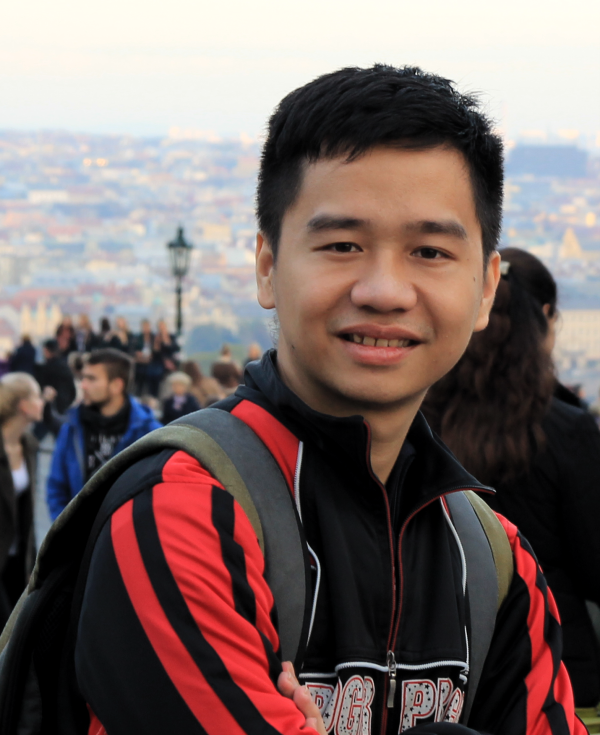
\includegraphics[width=2.5cm]{tamhd_2.png}
			%	\end{center}
			%\end{wrapfigure}
			
			\makechapter{Contact Information}
			
			\newlength{\rcollength}\setlength{\rcollength}{1.85in}%
			%
			\section{Name} 
			\textbf{Duc Tam Hoang}
			
			%\href{http://mff.cuni.cz/}{Mathematics and Physics Faculty, Charles University in Prague}
			Computational Linguistics Lab, National University of Singapore
			
			\ssection{Address}
			%527, Koleje Otava, Chemick\'a 954, Praha 4, Prague
			\# 05-407, Block 117, Lorong 1 Toa Payoh, 310117, Singapore
			
			\ssection{Personal Page}
			%527, Koleje Otava, Chemick\'a 954, Praha 4, Prague
			\href{http://tamhd.github.io}{http://tamhd.github.io}
			
			\ssection{Email}
			%\href{mailto:tamhd1990@gmail.com}{tamhd1990@gmail.com}
			\href{mailto:hoangdt@comp.nus.edu.sg}{hoangdt@comp.nus.edu.sg}
			
			%\href{mailto:tamhd1990@gmail.com}{tamhd1990@gmail.com}
			
			\ssection{Mobile}
			(+65) 90548590
			
			
			\makechapter{Education}
			
			\section{2013-2015}
			%
			\textbf{Charles University in Prague} \hfill Czech Republic
			
			\begin{innerlist}
				
				\item[] M.S, Computational Linguistics, Computer Science
				\begin{innerlist}
					%\item Faculty: Mathematics and Physics
					\item Graduate with honors
					\item GPA: 1.07 (\textit{excellent} - equivalent to 3.9 in the US 4.0 scale)
					\item Thesis: Pivoting Vietnamese Machine Translation System
				\end{innerlist}
			\end{innerlist}
			
			%\blankline
			
			\section{2008-2012}
			\textbf{University of Engineering and Technology, VNU} \hfill Vietnam
			
			\begin{innerlist}
				
				\item[] B.Sc, Computer Science (Honors Program)
				\begin{innerlist}
					%\item Program: International Standard Program
					\item GPA: 3.33/4.00 (\textit{Distinction})
					\item Thesis: An Ontology-based Vietnamese QA System for Academic Regulation
				\end{innerlist}
				
			\end{innerlist}
			\makechapter{Work/Research Experience}
			
			\section{2015-present}
			\textbf{National University of Singapore}
			\begin{innerlist}
				\item[] \textit{Research Assistant}%
				\begin{innerlist}
					\item Topic: Grammatical Error Correction
					\begin{innerlist}
						\item Analyze problems, devise solutions, implement systems and report results.
					\end{innerlist}
				\end{innerlist}
			\end{innerlist}
			
			
			\section{2014}
			\textbf{Institute of Formal and Applied Linguistics}, MFF, UK
			\begin{innerlist}
				\item[] \textit{Intern/Student}%
				\begin{innerlist}
					\item Topic: Statistical Machine Translation
					\begin{innerlist}
						\item Collect and clean parallel corpora
						\item Implement triangulation tools for Moses framework   
						\item Design SMT homework for ``MT talks'' (CodEx)
					\end{innerlist}
					%\item Advisor: Ond\v{r}ej Bojar (\href{mailto:ondrej.bojar@mff.cuni.cz}{ondrej.bojar@mff.cuni.cz})
				\end{innerlist}
			\end{innerlist}
			
			
			\section{2013-2014}
			%
			\textbf{TextAn - MFF automatic analysis of Police documents}, Prague
			
			\begin{innerlist}
				
				\item[] \textit{Developer - Software Project - MFF:  \href{https://github.com/PreXident/TextAn}{https://github.com/PreXident/TextAn}} 
				\begin{innerlist}
					\item Topic: Information Extraction
					\begin{innerlist}
						\item Implement Automatic Object Assigner: mapping natural entity to database object
						\item Integrate Machine Learning Classifier into a Java Project
					\end{innerlist}
				\end{innerlist}
			\end{innerlist}
			
			\section{2011-2013}
			\textbf{Human Machine Interaction Laboratory }, UET/Coltech, VNU
			\begin{innerlist}
				\item[] \textit{Research Assistant} \hfill In cooperation with Japan Advanced Institute of Science and Technology
				\begin{innerlist}
					\item Topic: Question Answering Systems (3 separated projects)
					\begin{innerlist}
						\item Create database in MySQL and Ontology OWL from text file
						\item Write rules/patterns for Vietnamese questions (in multiple domains)
						\item Implement maximum graph matching for QA system
					\end{innerlist}
					\item Topic: Information Retrieval System
					\begin{innerlist}
						\item Crawl data from forums and technical websites
						\item Cluster, index and query the collection using tools
					\end{innerlist}
				\end{innerlist}
			\end{innerlist}
			\vspace{.4\baselineskip}
			\begin{innerlist}
				\item[] \textit{Teaching Assistant} %\textit{Assistant Lecturer}%
				\begin{innerlist}
					\item Teach fundamental informatics for freshmen of Computer Science.
					\item Coach mathematics for the 21$^{st}$ Vietnam Mathematics Olympiad for Undergraduates.
					%\item Tutor students during office hours and lab sections, graded  weekly lab reports, graded exams and assignments.
				\end{innerlist}
			\end{innerlist}
			
			
			\section{2011}
			\textbf{Presentation Club}, UET, VNU
			\begin{innerlist}
				\item[] \textit{Organize club's meetings and events} %\textit{Assistant Lecturer}%
			\end{innerlist}
			
			\makechapter{Research Interests}
			\begin{innerlist}
				\item[] \textit{I am interested in topics of Computational Linguistics} %\textit{Assistant Lecturer}%
			\end{innerlist}
			
			\makechapter{Background/Skills}
			%
			\begin{innerlist}
				\item Background: Mathematics, Machine Learning, Computational Linguistics, Computer Science.
				\item Programming Languages: {\bf Python}, Perl, Shell Script, Java, C/C++.
				\item Tools: Git, Svn, Lucene, Carrot$^2$, Moses (inc. eman/ems), etc.
				\item Others: Regular Expression, Dynamic Programming, Object-oriented Programming, CSS/HTML/JSP. 
				\item Favorite Editor: vim
			\end{innerlist}
			
			\makechapter{Language Proficiency} 
			%
			\begin{innerlist}
				\item Vietnamese - native
				\item English - fluent
				\item Czech - basic
			\end{innerlist}
			
			\makechapter{Awards \& Honors}
			%
			
			\section{2014}
			\textbf{Excellence Scholarship} for top 1\% students at Faculty of Mathematics and Physics, Charles University in Prague.
			\vspace{-.6\baselineskip}
			\section{2013}
			\textbf{Fully-funded master scholarship} at Charles University in Prague. %{\scriptsize \textit{So far, I have been the only one who ever won this scholarship}}
			
			\vspace{-.6\baselineskip}
			
			\section{2010-2012}
			\textbf{1 First prize and 2 Second prizes} at Vietnamese National Mathematical Olympiad for Undergraduates.
			
			\textbf{Young Symbolization} award at University of Engineering and Technology.
			
			\textbf{Government Fellowship} for excellent students.
			
			\textbf{Excellent Academic Performance} at UET/Coltech.
			
			Rank \textbf{1$^{st}$} at the University Entrance Exam of UET/Coltech, VNU.
			
			
			\makechapter{Publications}
			
			\textbf{Published papers\footnote{There are also ``upcoming'' papers, please take a look at my full list of publications for more details}}
			\begin{enumerate}
				
				\item[6.] \underline{Duc Tam Hoang}, Shamil Chollamppattu and  Hwee Tou Ng. \textbf{Exploiting N-Best Hypotheses to Improve an SMT Approach to Grammatical Error Correction}. In Proceedings of the International Joint Conference on Artificial Intelligence, 2016.
				
				\item[5.] \underline{Duc Tam Hoang}and Ond\v{r}ej Bojar. \textbf{Data and Pivoting Methods for Czech-Vietnamese Translation via English}. In Proceedings of the 19th Annual Conference of the European Association for Machine Translation, 2016.
				
				\item[4.] \underline{Duc Tam Hoang} and Ond\v{r}ej Bojar. \textbf{TmTriangulate: A Tool for Phrase-Table Triangulation}. The Prague Bulletin of Mathematical Linguistics, 2015.
				
				\item[3.] Tung Xuan Vu, Minh Le Nguyen and \underline{Duc Tam Hoang}. \textbf{Semantic Parsing for Vietnamese Question Answering System}. In Proceedings of the 7th international conference on Knowledge and Systems Engineering, 2015.
				
				\item[2.] \underline{Duc Tam Hoang}, Minh Le Nguyen and Son Bao Pham. \textbf{L2S: Transforming natural language questions to SQL queries}. In Proceedings of the 7th international conference on Knowledge and Systems Engineering, 2015.
				
				\item[1.] Dat Tien Nguyen, \underline{Duc Tam Hoang} and Son Bao Pham. \textbf{A Vietnamese Natural Language Interface to Database}. In Proceedings of the 6th International Conference on Semantic Computing, 2012.
			\end{enumerate}
			
			\textbf{Others}
			\begin{enumerate}
				
				\item[2.] \underline{Duc Tam Hoang} and  Ond\v{r}ej Bojar. \textbf{CsEnVi Pairwise Parallel Corpora}. LINDAT/CLARIN digital library at Institute of Formal and Applied Linguistics, Charles University in Prague, 2015.
				
				\item[1.] \underline{Duc Tam Hoang} and  Ond\v{r}ej Bojar. \textbf{WMT 13 Test Set}. LINDAT/CLARIN digital library at Institute of Formal and Applied Linguistics, Charles University in Prague, 2015.
			\end{enumerate}
			
			%%(Under request)
			
			%%\begin{center}
			
			%%\tiny{Last updated: July 2012}
			%%\end{center}
			
			
		\end{document}
		
		%%%%%%%%%%%%%%%%%%%%%%%%%% End CV Document %%%%%%%%%%%%%%%%%%%%%%%%%%%%%
